\section{Ion Backflow and Gating}
\label{chap:TPC_sec:gating}
Most recent update: 2016-03-28 \\
Contact person: Akira Sugiyama (email: sugiyama@cc.saga-u.ac.jp)\\

\subsection{Introduction}

The distortion of particle tracks due to the accumulation of positive ions in the drift space is the well-known
issue for TPCs, whereby the ions are generated in the gas amplification region and drift back into the TPC drift volume.
Although this ion back flow is much suppressed for the MPGD technology, compared to the earlier MWPC TPCs, it can
still cause significant distortion of tracks when the particle density is high.

Because of the bunch-train structure of the ILC beams (i.e., a  train of ca. 1300 to 2600 bunches during
about \SI{1}{ms}
and a train-repetition rate of \SI{5}{Hz}), the ions flow back from the gas amplification and will form a few discs
of about \SI{1}{cm} thickness in the TPC drift volume where they slowly drift toward the TPC central cathode.
There will be three such ion discs during one train of normal ILC operation, and each disk will modify the trajectory
of the drifting electrons, resulting in the distortion of tracks. The simulations of this distortion at ILC
were made by several people, details can be found in \cite{LC-DET-2012-079,Fujii_IonEffects}.
Figure~\ref{Fig1gating} shows the azimuthal displacement of drift electrons by the ion
disks for different radial positions of TPC with three ion disks in the drift space at the drift distances
indicated by the red lines.

\begin{figure}
\begin{center}
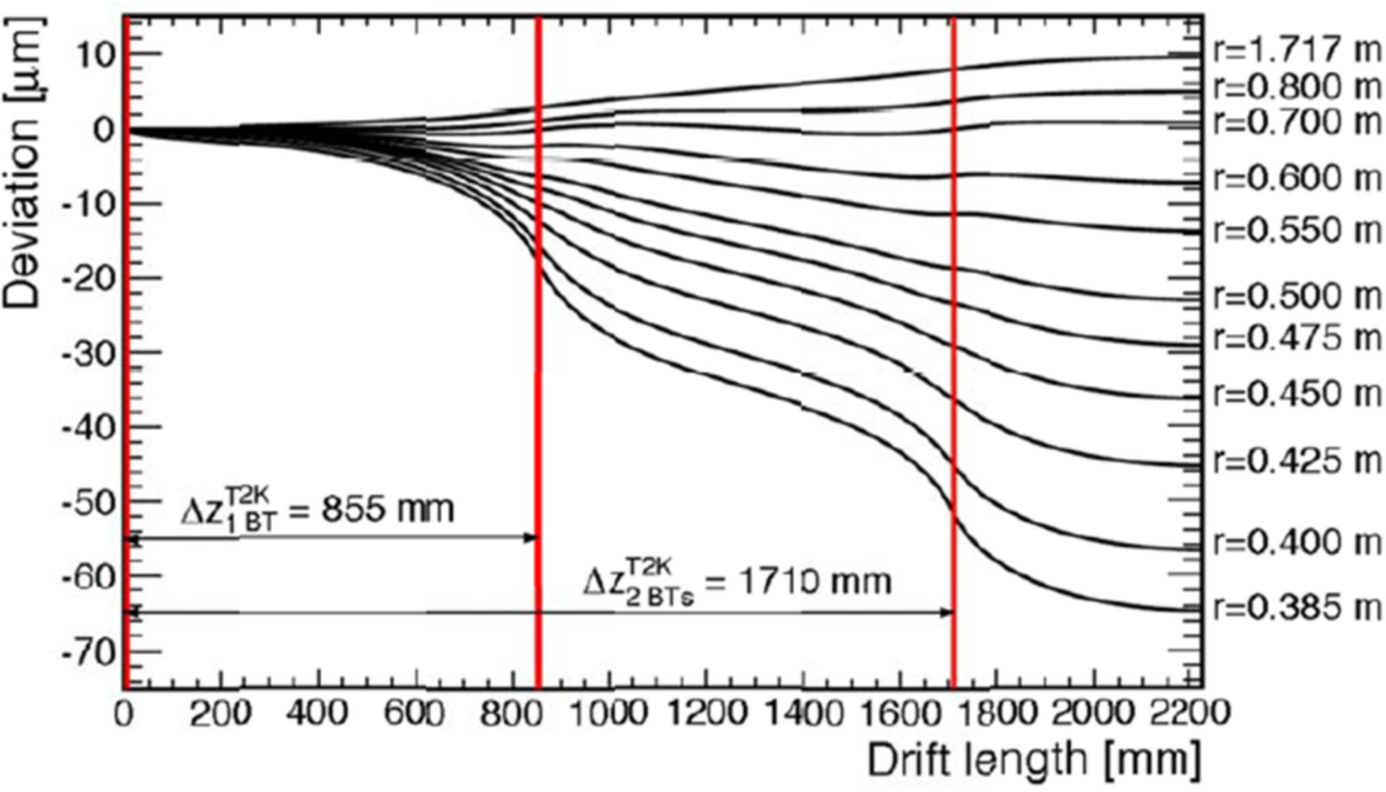
\includegraphics[width=.7\textwidth]{Tracker/TPC_Bonn/plots/TPC-Gate_Fig1gating.pdf}%
\caption{\label{Fig1gating} {Displacement due to the positive-ion discs.}}
\end{center}
\end{figure}


In  Fig.~\ref{Fig1gating} it is assumed that for every drift electron one positive ion drifts back.
The actual amount of displacement should therefore be multiplied by the ratio of the gas amplification
factor to the suppression factor of the ion backflow of the MPGD system. Since the suppression factor by the
MPGD system has been measured to be in the order of order 10$^{-3}$ at
best \cite{Fujii_IonEffects}, the ratio will be larger than one for a gas gain of a few thousand, and distortions larger
than \SI{60}{\micro m} in some parts of TPC would be expected.

At the ILC a TPC point resolution of \SI{100}{\micro m} or better is required by the physics. Thus it is
necessary to either install an efficient gating device to block the ions from the gas amplification, or to correct
the track distortion. Because the machine backgrounds at ILC may not be stable enough to make a reliable
correction possible, an efficient gating device will be needed. Fortunately the bunch-train configuration of ILC
has an ideal time structure for ion gating. The positive ions drift back around \SI{5}{mm} during
the \SI{1}{ms} bunch-crossing period, and can be absorbed by the ion gate which is `closed' (explanation
below) during next \SI{200}{ms} between the bunch trains.

For the expected particle density at ILC, the track distortion by the
{\em{primary}} ions produced in the LCTPC volume is small and has negligible effect.

\subsection{Engineering Challenges: a Wire Gate or a GEM Gate}

Ion gates used for TPCs in past collider experiments consisted of a wire grid. The operation and
structure of the wire gate is well known and can be used for the LCTPC. Figure~\ref{Fig2gating} shows
a simple mechanical prototype of such a wire gate mounted on an Asian GEM module.

\begin{figure}
\begin{center}
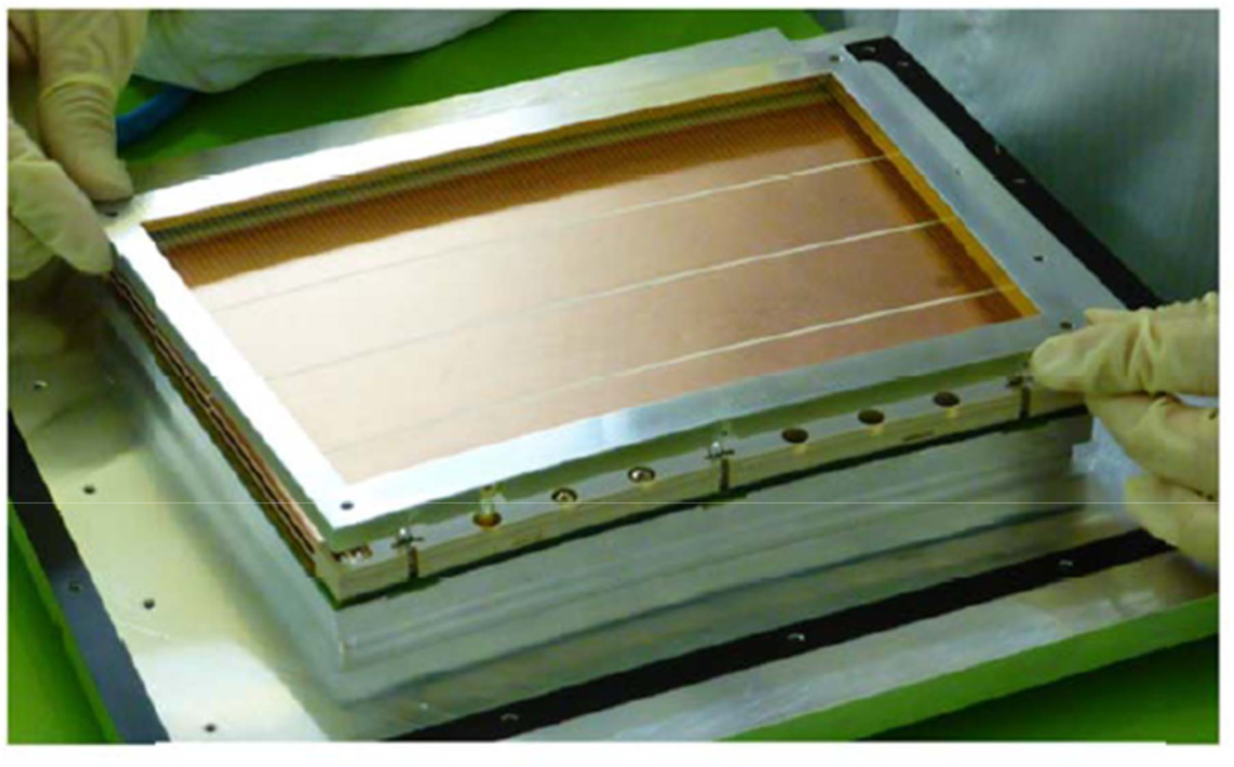
\includegraphics[width=.7\textwidth]{Tracker/TPC_Bonn/plots/TPC-Gate_Fig2gating.pdf}%
\caption{\label{Fig2gating} {Prototype wire gate installed on the Asian GEM module.}}
\end{center}
\end{figure}

The disadvantage of a wire gate for the LCTPC module is to deteriorate the advantages of an MPGD TPC:
the material and space budgets are increased because of the mechanical structure needed to support the many
stretched wires on the module. Therefore, the wire gate is kept as a backup option for the LCTPC, and efforts
are focused on the development of the gate using a GEM foil.

The idea of the GEM gate was proposed by F.~Sauli in 2006 \cite{Sauli2006269}.
The ions from the gas amplification have to be absorbed by the electrode of the gate-GEM in the gate-closed condition.
`Closed' is where the electric field across the gate-GEM is reversed by changing the potential of the bottom
electrode of the gate by about \SI{10}{V}. In the gate-open condition the drift electrons need to reach
to the gas amplification region with a high efficiency in order to not deteriorate the LCTPC resolution
due to loss of signal.

Details of the simulation of GEM gate using the Garfield++ may be found in \cite{LC-DET-2012-079}. Experience was that it is easy
to stop the ions with the necessary suppression factor of 10$^{-4}$ or smaller. On the other hand, it is more
of a challenge to keep a very high efficiency of the drift electrons passing through the gate-GEM in the gate-open
condition. This is because the efficiency is limited by the optical transparency of the gate-GEM when a TPC
is used in a high magnetic field (as in the \SI{3.5}{T} field of ILD) and with a high-$\omega\tau$ gas mixture,
such as the T2K gas \cite{Behnke:2013lya,ref4T2Kgas_ishikawa,Kobayashi201137,Kobayashi2013122} foreseen for the LCTPC. In this condition the drift electron tends to follow the
magnetic field lines rather than the electric field lines, which makes the optical transparency an important parameter .

The first GEM gate prototype for the Asian GEM module for the TPC large prototype (LP) beam test at
DESY in 2009 was \SI{14}{\micro m} thick with the round GEM holes of
\SI{90}{\micro m} diameter and \SI{140}{\micro m} pitch. It had a maximum electron
transmission of 50\% in the magnetic fields of \SI{1}{T} and \SI{0}{T}. It was clear that a GEM
with bigger holes and a narrow rim was needed, that is with larger optical transparency. Simulations found that
GEM holes of the honeycomb shape with very thin rims would maximize the optical transparency.

\begin{figure}
\begin{center}
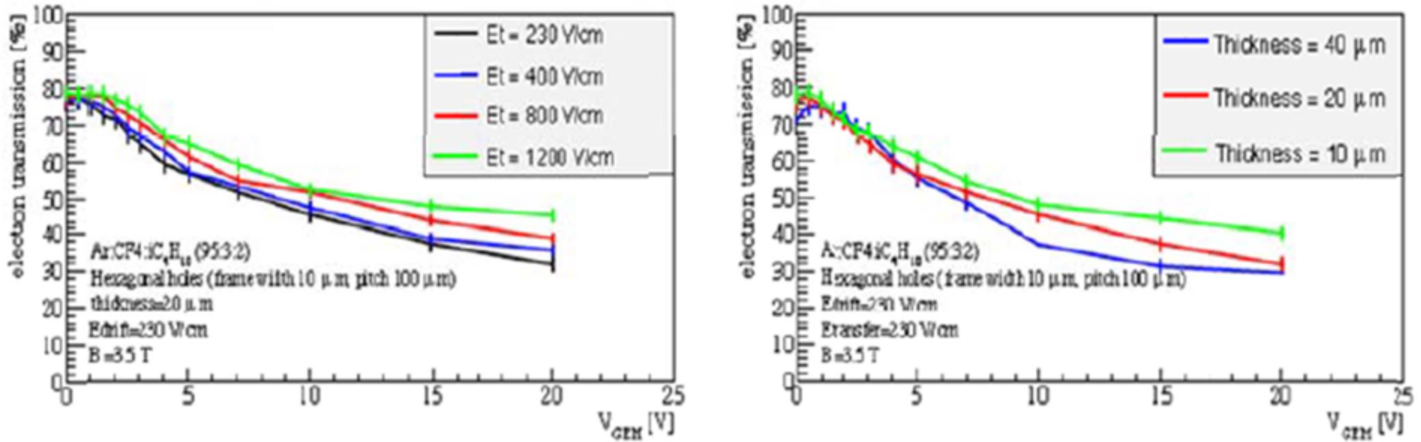
\includegraphics[width=.7\textwidth]{Tracker/TPC_Bonn/plots/TPC-Gate_Fig3gating.pdf}%
\caption{\label{Fig3gating} {The electron transmission simulated for a gate-GEM with the honeycomb-shaped holes of pitch \SI{100}{\micro m} and rim width \SI{10}{\micro m}.}}
\end{center}
\end{figure}

As is seen the simulation results shown in Fig.~\ref{Fig3gating}, the thin gate GEM with
honey\-comb-shaped holes of \SI{100}{\micro m} pitch and \SI{10}{\micro m} rim width is shown to reach
an electron transmission of 80\%. However, a rim width of \SI{10}{\micro m} turns out to be very difficult to produce;
an alternative is presented in the next subsection.

\subsection{Recent Milestones}

In 2013 the Japanese LCTPC group started the actual fabrication of the GEM gate with the large
optical transmission. With the limitations of the available processes of GEM, the specifications
were set using  Fig.~\ref{Fig45gating}(lower)
which are summarized in the Table 1. The target is to fabricate a gate GEM with  honeycomb shape holes
of around \SI{300}{\micro m} diameter and  rim-width of \SI{35}{\micro m} or smaller. The immediate goal
of this study is to test the Asian LP module with this GEM gate in the DESY test beam in 2016.

\begin{table}
\begin{center}
\begin{tabular}{|l|l|}
\hline
Item & Specification \\%$\sim$
\hline
\hline
Optical aperture ratio &  80\% \\
Hole size       & \SI{300}{\micro m}\\
Hole pitch       & \SI{335}{\micro m}\\
Rim size            & \SI{35}{\micro m}  \\
Insulator thickness  & \SI{25}{\micro m}\\
Foil size            & $170\times\SI{220}{mm}$ \\
\hline
\end{tabular}
\caption{\label{gatespecs} Specification of the gate-GEM in the current study.}
\end{center}
\end{table}

Prior to the fabrication of a large, module-sized gate, many small samples of
\SI{10}{cm} $\times$ \SI{10}{cm} were produced to test different processing techniques.
Although some samples by the standard single-mask chemical process were promising, limited resources required that
a major effort be continued with Fujikura Ltd.~\cite{ref5fujikuraltd} using their laser-chemical hybrid technology to produce
FPCs (flexible printed circuits). Details of the Fujikura process for the gate-GEM were presented at MPGD2015 \cite{MPGD2015_gate}.
Figure~\ref{Fig45gating}(upper) shows the structure of one of the gate-GEM small samples made by Fujikura
according to the specifications in Table \ref{gatespecs}.

\begin{figure}
\begin{center}
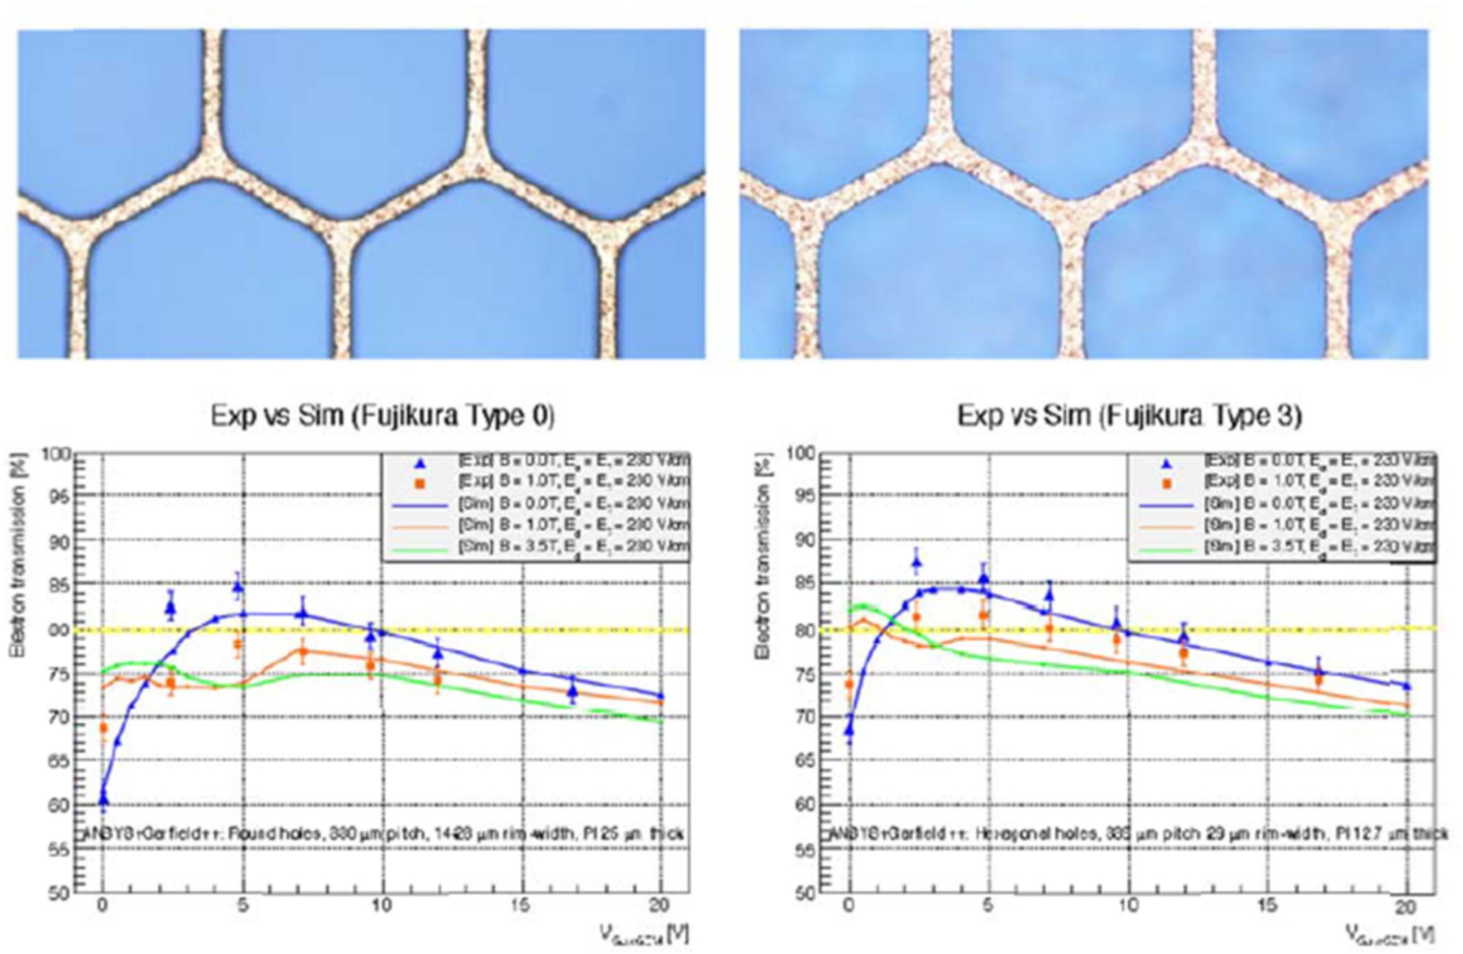
\includegraphics[width=.7\textwidth]{Tracker/TPC_Bonn/plots/TPC-Gate_Fig45gating.pdf}%
\caption{\label{Fig45gating} {Upper: Honeycomb hole structure of the gate-GEM.
The pitch of the holes is \SI{335}{\micro m}, the rim width \SI{29}{\micro m}.
The polyimide insulator is \SI{12.7}{\micro m} thick.
Lower: Preliminary results of the electron transmission measurement are compared to simulation
as functions of the GEM voltage for two types of gate-GEMs. In the left panel are
results for gate-GEM with round holes; in the right panel results for the gate-GEM with the honeycomb-shaped holes.}}
\end{center}
\end{figure}

The electron transmission was measured for these samples, and
Fig.~\ref{Fig45gating}(lower) shows the results of the measurement compared to the simulation in magnetic fields
of 0, 1 and \SI{3.5}{T}. In the left panel, the results for the sample with round holes, and in the right panel
for the sample with honeycomb-shaped holes.  The electron transmissions at 0 and \SI{1}{T} were confirmed
to be better than 80\% while the optical transmission was calculated to be 82\% for the honeycomb-shaped-hole sample.

Having established the best configuration and the best process for the gate GEM with the small samples,
the focus has now moved to the fabrication of the gate-GEM with  the size of the Asian GEM module (Fig.~\ref{Fig6gating}).
Here the major issue for the fabrication is to minimize any defects in the electrode circuit of the gate-GEM
so that there is 100\% stopping power of the ions.

\begin{figure}
\begin{center}
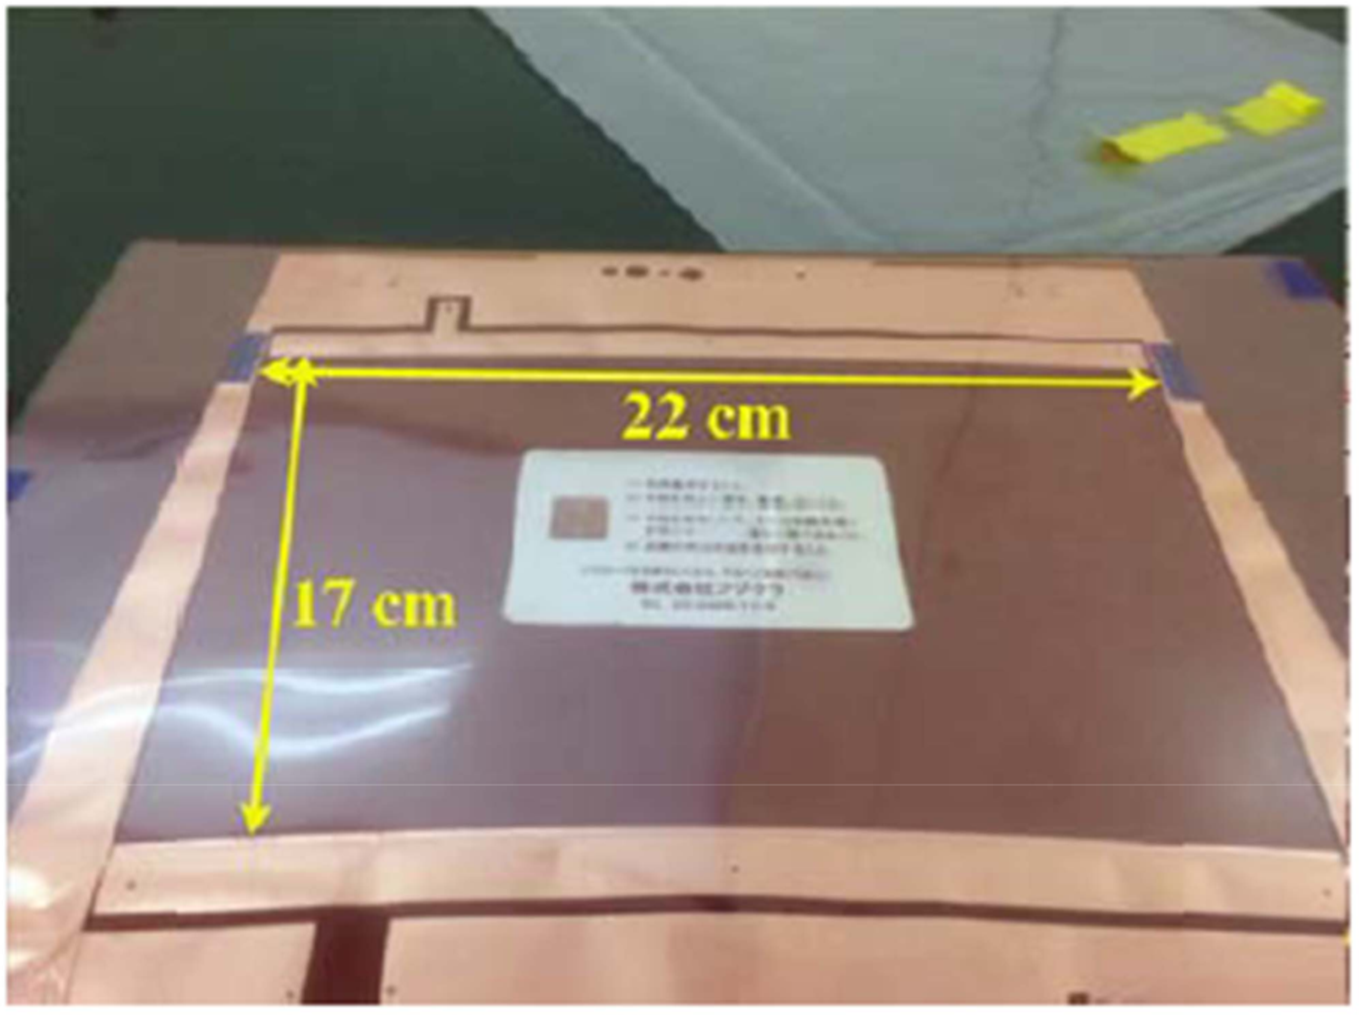
\includegraphics[width=.7\textwidth]{Tracker/TPC_Bonn/plots/TPC-Gate_Fig6gating.pdf}%
\caption{\label{Fig6gating} {A sample gate-GEM for the Asian module.}}
\end{center}
\end{figure}

\begin{figure}
\begin{center}
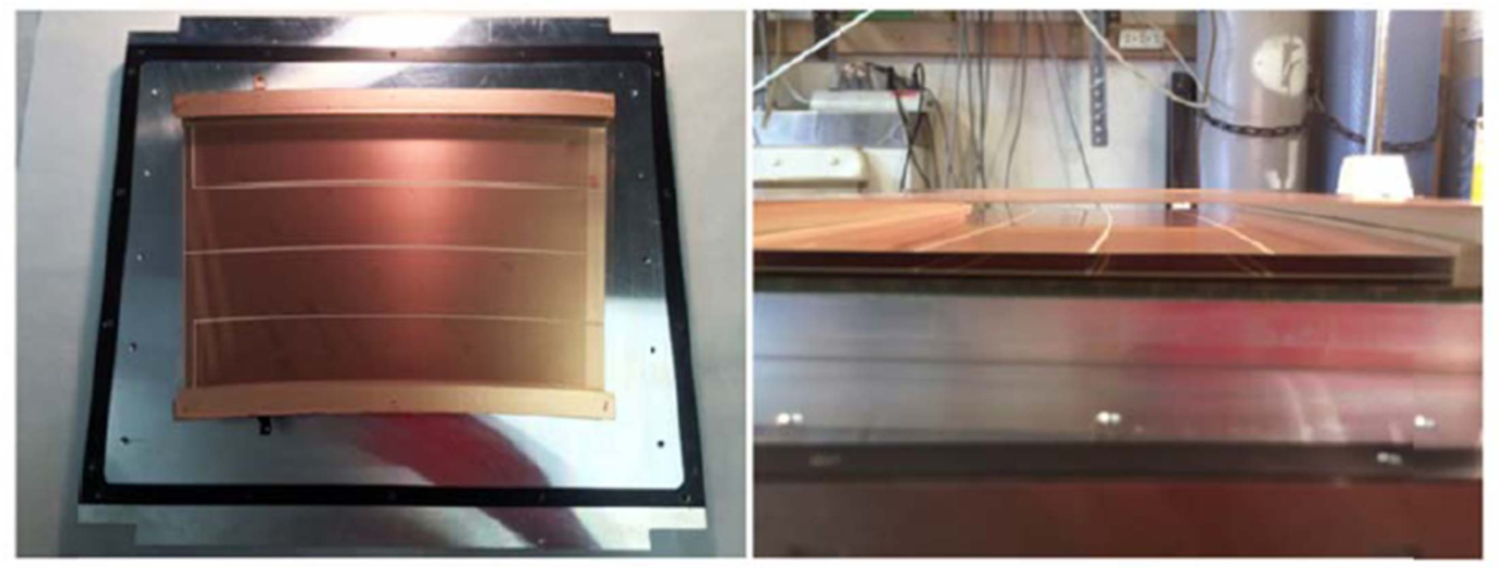
\includegraphics[width=.7\textwidth]{Tracker/TPC_Bonn/plots/TPC-Gate_Fig78gating.pdf}%
\caption{\label{Fig78gating} {Left panel: Test mounting of the gate-GEM. Right panel: Test assembly of the gate GEM on the Asian GEM module.}}
\end{center}
\end{figure}

Figure~\ref{Fig78gating}(left) shows the test mounting of the gate-GEM on the module. As can be seen,
the pattern of the amplifier GEM below the thin gate-GEM can be seen clearly, indicating a  high optical transparency.
Figure~\ref{Fig78gating}(right) is a picture of a test assembly of the gate-GEM on the module.

\subsection{Future Plans}

The production process for the large gate-GEM has been essentially established,
and a few of the good samples for the Asian GEM module have been delivered for testing.
The preparations for measuring the electron transmission by using a laser beam are under way.
Although the Asian model is designed to have a GEM gate mounted on it,
there may be more issues coming up, and some optimization of the mounting method and the module structure
might become necessary for the design of the LCTPC. Beside some difficulties to stretch such a thin
GEM stably, some consideration on the possible ion leak through the module boundaries
for the Asian GEM modules may be needed.
